%\documentclass[letter paper,10pt]{article}
%\usepackage{float}
%\begin{document}
\marginparwidth = 1in
\marginparpush = 0pt
\voffset = 0pt
\paperheight = 11in

\section{Introduction to Enhanced IP}
The Enhanced IP (EnIP) design increases IP address space.
EnIP allows up to approximately 2\textasciicircum 56 possible addresses 
in contrast to IPv6's offer of approximately 2\textasciicircum 128 addresses. 
The word approximately is used since both protocols include a few address 
ranges not available for use.  EnIP also offers a very practical path towards 
wide scale adoption.  It is this upgrade path and similarity to the existing IPv4
model that many may find valuable.

EnIP uses IP option 26 to create a twelve byte extension to the IP header.  This extension contains four bytes of overhead, 
and two four byte fields used as additional storage for the EnIP source and destination addresses.  
EnIP addresses are written as two IPv4 addresses concatenated together.

\subsection{EnIP Addressing Example}
An EnIP host addresses another EnIP host as follows:

\begin{center} 
65.127.221.2.10.1.1.2
\end{center}

\begin{enumerate}

\item In this example, 65.127.221.2 is a public IPv4 address allocated 
by one of the Internet registries.  Under EnIP, this address is called the site address.

\item 10.1.1.2 is a private IPv4 address assigned to a host behind a 
NAT.  In this case, the NAT and the host behind it have been upgraded to include
software to handle the EnIP extension to IPv4.

\item On the public IPv4 network, 65.127.221.2 is used for routing purposes.  In other words,
while the packet traverses the public network, its IPv4 destination is 65.127.221.2.  
Once the packet reaches 65.127.221.2, which is a NAT upgraded with EnIP software, the IPv4 
destination address is changed to 10.1.1.2, which is a value stored in the additional 12 bytes 
of space afforded by IP option 26.  The byte layout used for IP option 26 is defined in Figure 1.
\end{enumerate}

\subsection{IP Header with EnIP Option Header}
This is the IPv4 header along with additional space used 
by IP option 26\cite{rfc791}.
%\begin{center}
%\begin{figure}[H]
%\begin{verbatim}
%   0                   1                   2                   3
%   0 1 2 3 4 5 6 7 8 9 0 1 2 3 4 5 6 7 8 9 0 1 2 3 4 5 6 7 8 9 0 1
%  +-+-+-+-+-+-+-+-+-+-+-+-+-+-+-+-+-+-+-+-+-+-+-+-+-+-+-+-+-+-+-+-+
%1 |Version|  IHL  |Type of Service|          Total Length         |
%  +-+-+-+-+-+-+-+-+-+-+-+-+-+-+-+-+-+-+-+-+-+-+-+-+-+-+-+-+-+-+-+-+
%2 |         Identification        |Flags|      Fragment Offset    |
%  +-+-+-+-+-+-+-+-+-+-+-+-+-+-+-+-+-+-+-+-+-+-+-+-+-+-+-+-+-+-+-+-+
%3 |  Time to Live |    Protocol   |         Header Checksum       |
%  +-+-+-+-+-+-+-+-+-+-+-+-+-+-+-+-+-+-+-+-+-+-+-+-+-+-+-+-+-+-+-+-+
%4 |                Source Host Number                             |
%  +-+-+-+-+-+-+-+-+-+-+-+-+-+-+-+-+-+-+-+-+-+-+-+-+-+-+-+-+-+-+-+-+
%5 |              Destination Host Number                          |
%  +-+-+-+-+-+-+-+-+-+-+-+-+-+-+-+-+-+-+-+-+-+-+-+-+-+-+-+-+-+-+-+-+
%6 |             |              |E|E|                              |
%  |  Option ID  |     Option   |S|D|       Reserved               |
%  |      0X9a   |     Length   |P|P|                              |
%  +-+-+-+-+-+-+-+-+-+-+-+-+-+-+-+-+-+-+-+-+-+-+-+-+-+-+-+-+-+-+-+-+
%7 |                      Enhanced IP Source Address               |
%  +-+-+-+-+-+-+-+-+-+-+-+-+-+-+-+-+-+-+-+-+-+-+-+-+-+-+-+-+-+-+-+-+
%8 |                   Enhanced IP Destination Address             |
%  +-+-+-+-+-+-+-+-+-+-+-+-+-+-+-+-+-+-+-+-+-+-+-+-+-+-+-+-+-+-+-+-+
%\end{verbatim}
%\caption{The EnIP Packet}
%\label{Figure 2}
%\end{figure} 
%\end{center}


\begin{figure}[H]
\begin{center}
\caption{Header}
\label{Figure 1}
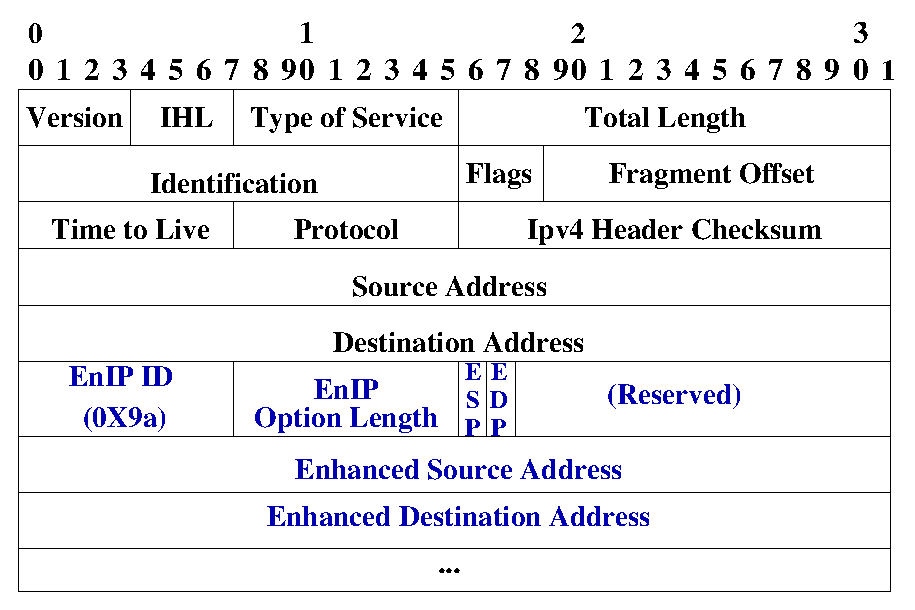
\includegraphics[scale=.5]{images/EnIPHdr.eps}
\end{center}
\end{figure} 


The EnIP ID field contains the value 0X9a.   This field can be broken down further
by converting the hexadecimal value 0x9a to binary:

\begin{center}
\textbf{1 00 11010}
\end{center}

\begin{enumerate}
 \item The first bit is a 1.  This represents the copy bit.
 \item The next two digits are 00.  This represents the \textbf{control} Option Class.
 \item The next five digits are 11010, or 26 in base 10.  This represents the new IP option value.
\end{enumerate}


If an EnIP packet traverses a router and must be fragmented because 
of a link with a smaller MTU, the copy bit ensures that fragments
include the 12 byte IP option header in each of the fragmented
packets.

In EnIP, the second byte after 0x9a is the Option Length.  This value
is always 12.  ESP and EDP are one bit fields used to indicate
whether EnIP Source Address and EnIP Destination Address are in use.
The Reserved field is unused and always set to zero.

%\begin{center}
%\begin{figure}[H]
%\begin{verbatim}
%      copy bit      Option Class          Option Value
%   +-------------+------------------+-----------------------+
%   |     1       |        00        |         01010         |
%   +-------------+------------------+-----------------------+
%   |copy bit set | Class is Control | Option is a new value |
%   +-------------+------------------+-----------------------+
%\end{verbatim}
%\caption{The EnIP Option Field}
%\label{Figure 2}
%\end{figure}
%\end{center}


The following scenarios describe the operation of EnIP, but first describe several IPv4 scenarios 
that exist today as part of a build up to help the Internet community understand the 
changes required to implement EnIP. 

Reference Figure 2 in the scenarios described below:

\begin{figure}[H]
%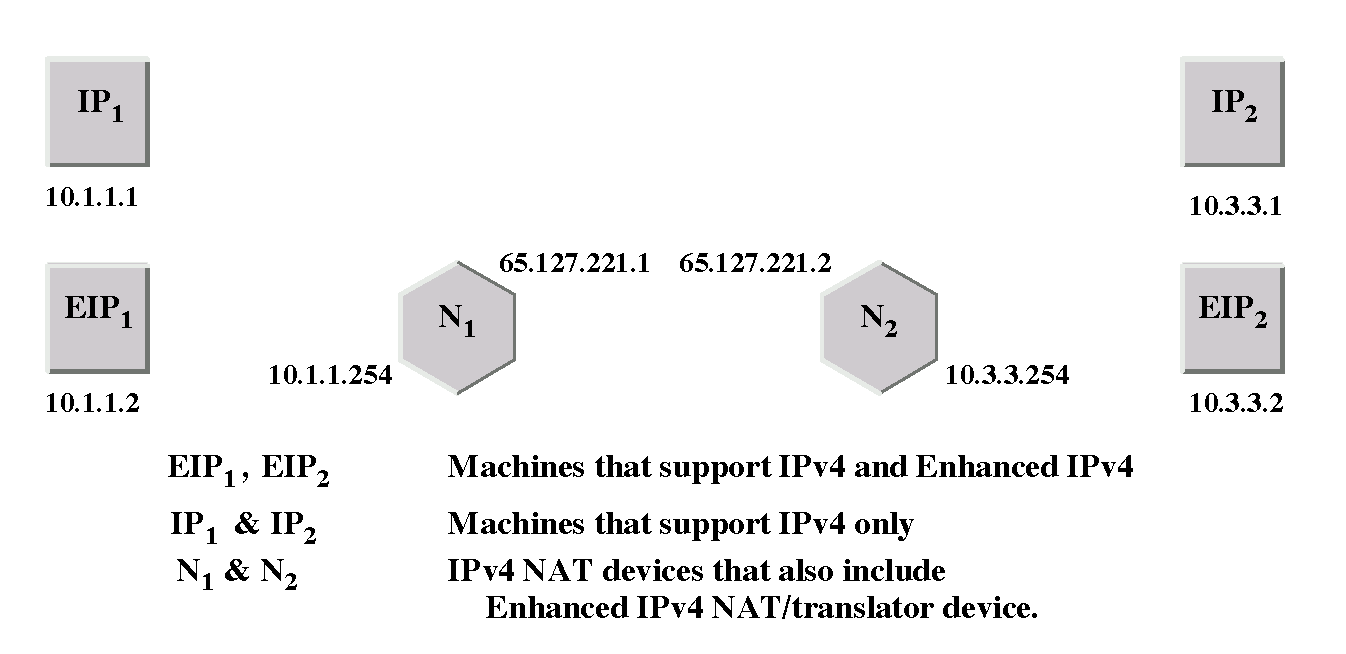
\includegraphics[scale=.7]{images/EnIPnodes.eps}
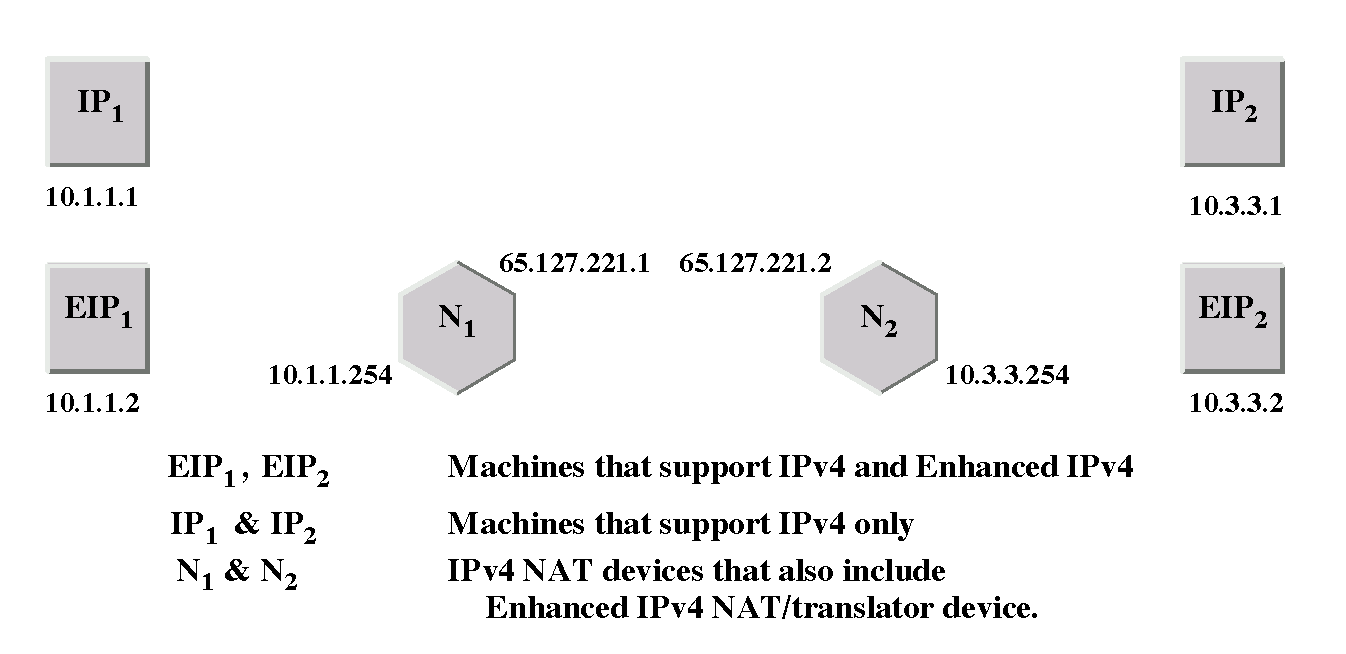
\includegraphics[height=3.0in]{images/EnIPnodes.eps}
\caption{IPv4 and Enhanced IPv4 co-existence}
% \label{fg:Xname2}
\label{Figure 2}
\end{figure}


\subsection{NAT Explanation using Figure 2}
\begin{enumerate}
 \item When IP1 (10.1.1.1), which is a host with an IPv4 stack, wants to reach 65.127.221.2 it 
  uses NAT to masquerade as the public IP address 65.127.221.1. 
  (Port-restricted cone NAT as on Linux iptables).

 \item Suppose IP1 (10.1.1.1) wants to reach tcp port 80 on IP2 (10.3.3.1), 
the packets originating from 10.1.1.1 are NAT'd by N1 to use a source IP 
address of 65.127.221.1. When these packets arrive at N2 (65.127.221.2), it is necessary 
to have a NAT port forwarding rule setup on N2 to map tcp port 80 on 65.127.221.2 
to forward packets to the internal host IP2 (10.3.3.1). This example nicely 
illustrates the power of NAT but also highlights the weaknesses of NAT to 
enable end to end host connectivity.

 \item EIP1 is a host with an IPv4 software 
stack as well as Enhanced IP extensions to IPv4. EIP stands for "Enhanced IPv4". 
Suppose EIP1 (10.1.1.2) wants to reach N2 (65.127.221.2). In this case, the 
destination IP address EIP1 will talk to is an IPv4 address (65.127.221.2). 
Because of this, the NAT device (N1) uses IPv4 NAT to translate the 
source of the packets to come from 65.127.221.1. In this case, EIP1 
behaves as though it is an IPv4 host as there is no need to use EnIP.

 \item Suppose EIP1 (10.1.1.2) wants to reach IP2 (10.3.3.1) on 
tcp port 80. In order to reach IP2, it is necessary to talk to 
N2 on address 65.127.221.2. Since this is also a function that can 
be satisfied by IPv4, when the packets from EIP1 reach N1 they 
are translated to appear as though they are coming from N1's 
external IPv4 address of 65.127.221.1. When the packets from 65.127.221.1 
reach 65.127.221.2, 65.127.221.2 must have a port forwarding entry for 
port 80 setup to send the packets to IP2 (10.3.3.1). 
It is important to note that thus far we have not demonstrated 
any usage of Enhanced IPv4 features.
\end{enumerate}

\subsection{EnIP Explanation using Figure 2}

\begin{enumerate}
\item Suppose EIP1 wants to send packets to EIP2. In this instance both hosts are running Enhanced IPv4 stacks and it is assumed that N1 and N2 support EnIP. Suppose EIP1 knows the address of EIP2 is 65.127.221.2.10.3.3.2 (more on DNS later). EIP1 knows its internal IP address of 10.1.1.2 but is not aware of the external address of N1 (65.127.221.1). Thus, initially the following is done: 
  \begin{itemize}
   \item The source IPv4 address is set to the address 10.1.1.2.
   \item The EnIP ID field is set to 0X9a.
   \item The ESP bit in the EnIP header is set to zero. 
   \item The Enhanced IP Source Address in the EnIP header is set to all ones, or 255.255.255.255, since an Enhanced IP source address is not currently present.
   \item The most significant 32 bits of the EnIP address is set by storing 65.127.221.2 in the IPv4 destination field 
   \item The least significant 32 bits of the EnIP address is set by storing 10.3.3.2 in the Enhanced IP Destination Address field.
   \item The EDP bit is set to 1.
  \end{itemize}

\item When the packet arrives via IPv4 routing to N1, N1 does the following:
  \begin{itemize}
  \item Examines the packet and determines it has the Enhanced IP options present (0x9a). 
  \item Writes the EnIP source address by reading 10.1.1.2 from the IPv4 source address field and
  placing this value in the Enhanced IP Source Address field.  This field no longer contains 255.255.255.255.
  \item  Sets the ESP bit to 1.
  \item  Places 65.127.221.1 as the IPv4 source address.
  \item  Recomputes the IP checksum of the packet since it has changed.  If the packet carries TCP or UDP, recomputes these checksums as they have also changed.
  \end{itemize}
\item Upon arrival at N2 (65.127.221.2), N2 does the following:
  \begin{itemize}
  \item Recognizes the Enhanced IP packet. (0x9a)
  \item Reads the EnIP Destination Address of 10.3.3.2 and places this value into the IP header's destination address, so that the IP destination address is now 10.3.3.2.
  \item Sets the EDP bit to 0
  \item Sets EnIP Destination Address to zero.
  \item Recomputes the IP checksum.  If the packet carries TCP or UDP, recomputes these checksums as they have changed as a result of a change to the IP destination address.
  \item N2 sends the packet to EIP2.
  \end{itemize}

  \item When EIP2 receives the packet it does the following:
  \begin{itemize}
   \item Computes the source address of the packet by concatenating the 
  IPv4 source field (65.127.221.1) with the EnIP source field (10.1.1.2) to get 65.127.221.1.10.1.1.2.
  \item The IPv4 destination address is 10.3.3.2.
  \end{itemize}

\item To construct a packet from EIP2 to EIP1, EIP2 does the following:
  \begin{itemize}
   \item  Sets the Option ID field to 0x9a.
   \item Takes the IPv4 source address field from the incoming packet, 65.127.221.1,
   and sets it as the IPv4 destination field.
   \item  Places the EnIP source address (10.1.1.2) in the EnIP Destination Address field.
   \item Set the EDP field to 1.
   \item  Sets the IPv4 source address field to 10.3.3.2.
   \item  Sets the EnIP source address to all ones (255.255.255.255), setting the ESP bit to 0.
  \end{itemize}

\item When the packet arrives at N2, the following is done by N2:
  \begin{itemize}
   \item Places 10.3.3.2 in the EnIP source address field.
   \item Set the ESP bit to 1.
   \item Place 65.127.221.2 in the IPv4 source address field.
   \item Recomputes the IP checksum and if the packet carries TCP or UDP, recompute these checksums as well.
   \item Send the packet to N1 (65.127.221.1).
  \end{itemize}

\item When the packet arrives at N1, it does the following:
  \begin{itemize}
   \item  Read 10.1.1.2 from the EnIP destination address field, and place this value in the IPv4 destination address field.
   \item  Set EDP to 0.
   \item Place a value of 0 in the EnIP destination address field.
   \item Recompute the IP checksum and if the protocol is TCP or UDP, recompute these checksums as well.
   \item Send the packet to EIP1..
  \end{itemize}

\end{enumerate}

\subsection{Upgrading Servers to Support EnIP}
An existing server deployed using an IPv4 address can be easily upgraded to support EnIP connections.
Suppose the server is a simple TCP echo server\cite{rfc862}.  The echo program creates a listening socket and then reads data from it.
Any data read from the socket is also written back to the same socket.  Without being upgraded, it should
be possible for the server to read EnIP packets from the socket.  However, it will not be possible for the server
to write EnIP packets back to the socket correctly.  The packets would only be sent to the source IPv4 address and not
back to the EnIP address which includes the source IPv4 address and the EnIP Source Address.  Once the server
has the EnIP upgrades, it will be possible for it to receive packets and send echo responses back to the full EnIP 
address that originated the packet.  Care must be taken here to ensure that the EnIP Source Address is one of the 
allowed RFC 1918 addresses.  

Suppose the echo server also logs the source IP address of each data packet received using the \textit{getpeername}
function.  The length of the address structure returned is currently either the size of a \textit{struct sockaddr\_in} (16 bytes) for IPv4
or the size of \textit{struct sockaddr\_in6} (28 bytes) for IPv6.  The ALPHA implementation of EnIP returns a new structure called
\textit{struct sockaddr\_ein}(26 bytes).  If it is desired to print out the EnIP addresses correctly, it is necessary to 
use the length 26 to detect a \textit{struct sockaddr\_ein}.  Inside this struct are two values: sin\_addr1 and sin\_addr2.  These
represent the IPv4 source address and the EnIP Source Address.  An implementation of getpeername could provide a compatibility
mode to treat EnIP addresses as IPv4 addresses.  Once the echo client software is upgraded, the getpeername implementation could
return struct sockaddr\_ein.

\subsection{DNS Operation}
RFC 2928 sets aside\cite{rfc4727} the experimental IPv6 prefix 2001:0101.  
EnIP lookups use AAAA records that begin with the experimental prefix 2001:0101.  
The prefix 2001:0101 uses 32 bits of the 128 bit AAAA record, leaving 96 bits for EnIP to 
use, of which 64 bits are used.
Supposing the EnIP address was 65.127.221.2.10.1.1.2, the EnIP AAAA record would be 2001:0101:417f:dd02:0a01:0102::0.
This use of the AAAA record is called a AA record.  It is important to note that a new AA record type was not added, rather
the AA record is a record created by retrofitting the 64 bit EnIP address into the existing AAAA record.  
With this approach, it is not necessary to upgrade DNS server software so long as it supports AAAA lookups.
It is imagined in the future, that DNS software will be upgraded to hide these details from the user.  For example,
the user might enter:

\begin{verbatim}
65.127.221.1.10.1.1.2       AA       eip1.example.com
65.127.221.2.10.3.3.2       AA       eip2.example.com
\end{verbatim}


\subsection{Optional DNS Upgrades}
Suppose EIP1 must speak to another EIP host behind N1.
Call this host EIP3. EIP3 has an address of 10.1.1.3 and like EIP1 has an 
external source address of 65.127.221.1. An important question to consider is can EIP1 talk 
to EIP3 using EnIP addressing without relaying all packets via N1?  Suppose the enterprise uses the domain name
example.com.  On the authoritative name server for example.com, the enterprise maintains a list of IP networks controlled by the
enterprise.  Suppose 65.127.221.1 is the only entry in the list.  DNS resolvers typically look up AAAA records followed by A records
if the AAAA lookup does not succeed.  If a DNS query from 65.127.221.1 arrives at the authoritative server requesting a AAAA record
for EIP3.example.com it would be possible to send back DNS answer for no such record.  When the request for the A record for EIP3.example.com
arrives at the name server, the authoritative server responds with the least significant 32 bits of the EnIP address.  When other
IP addresses query the authoritative name server asking for the AAAA record of EIP3.example.com, they will receive the EnIP address encoded as an IPv6 address.

\subsection{Security Issue: Preventing EnIP NAT or hosts from forwarding illegal packets}
EnIP-capable NAT devices swap the EnIP destination address into the IPv4 header's destination address.  Once the swap occurs the packet
is routed on to the address stored in the EnIP destination field.  This is the desired behavior when the destination address is for a network directly connected
to the NAT.  This is not the desired behavior if the NAT is forwarding on to a network that is not directly connected.  EnIP NAT devices MUST only perform
the swap and forward operation if the EnIP destination address is for an RFC 1918 address of a network directly connected to the EnIP NAT.  
To perform this swap otherwise, would mean packets sent to EnIP NATs could be used to relay packets towards
unwitting victims.  If not protected against, this could lead to these packets being used in denial of service attacks or other malicious acts.

\subsection{Security Issue: IPSEC}
EnIP breaks IPSEC in the full tunnel mode AH+ESP scenario.  NAT
already breaks this configuration of IPSEC. It is important to acknowledge this as a design limitation.  More work would be required to
modify IPSEC to work with EnIP.  

\subsection{Security Issue: Host security, sensible defaults}
EnIP hosts behind a permissive EnIP NAT device are more exposed on the Internet.  It is recommended that the default configuration
of an EnIP NAT not allow any inbound connections to EnIP hosts behind the NAT unless explicitly configured to do so.  This is the most sensible configuration
for EnIP devices designed for the home user as replacements/upgrades to existing NAT gateways.  This configuration will not be possible for the
mobile network.

%\end{document}
